\documentclass[12pt,a4paper]{article}

\usepackage[margin=25mm,headheight=15pt]{geometry}
\usepackage[T1]{fontenc}
\usepackage[utf8]{inputenc}
\usepackage{amsmath,amssymb,mathtools}
\usepackage{booktabs,array,multirow}
\usepackage{graphicx}
\usepackage[dvipsnames]{xcolor}
\usepackage{tikz}
\usetikzlibrary{calc,arrows.meta}
\usepackage{pgfplots}
\pgfplotsset{compat=1.18}
\usepackage[colorlinks=true,linkcolor=blue!60!black,citecolor=blue!60!black]{hyperref}
\usepackage{pifont}
\usepackage{siunitx}
\usepackage{caption}
\usepackage{fancyhdr}
\usepackage[numbers,sort&compress]{natbib}
\usepackage{enumitem}
\usepackage{float}

\definecolor{sambpblue}{RGB}{0,70,140}
\definecolor{okgreen}{RGB}{0,140,60}
\definecolor{warnred}{RGB}{180,20,20}

\pagestyle{fancy}
\fancyhf{}
\lhead{\textcolor{sambpblue}{\textbf{SAMBP TR-11/2026}}}
\rhead{HIF Sensitivity Margin Study}
\cfoot{\thepage}

\newcommand{\SAMBP}{\textsc{sambp}}
\newcommand{\kappan}{\kappa_{\rm n}}
\newcommand{\fint}{f_{\rm int}}
\newcommand{\Iop}{I_{\rm op}}
\newcommand{\Iopmin}{I_{\rm op,min}}

\begin{document}

\begin{center}
  {\LARGE\bfseries\color{sambpblue}
    SAMBP Technical Report TR-11/2026}\\[6pt]
  {\large High-Impedance Fault Sensitivity Margin Study:\\
    Minimum Detectable Fault Current for Each Protected Zone}\\[10pt]
  {\normalsize PhD Thesis Supporting Report \quad|\quad
    Revision~1.0 \quad|\quad 3 April 2026}
\end{center}

\vspace{4pt}\hrule\vspace{8pt}

\begin{abstract}
\noindent
This report characterises the minimum detectable fault current for each
\SAMBP{} protected zone by sweeping a scale factor $\alpha \in
[1.00,\,0.05]$ on the nominal fault current and evaluating trip
probability over 200~trials per level.  Nine $\alpha$ levels are tested
across ten relay--scenario combinations.  The study reveals a fundamental
sensitivity--specificity trade-off inherent in the Stage-2 confidence
gate: bus differential (87B) and transformer differential (87T) zones
maintain TPR~=~1.000 down to $\alpha = 0.05$ ($I_f \geq 0.20$~pu), but
the line differential (87L) Stage-2 gate raises the effective detection
threshold to $I_f \approx 0.72$~pu (Phase-to-Ground) or 0.56~pu
(Three-phase) — 3--4$\times$ above the conventional relay's effective
threshold of 0.20--0.24~pu.  The over-current (OC) relay detection
margin follows the pickup threshold analytically.  These results quantify
the selectivity--sensitivity trade-off and provide zone-specific
detection margin tables for the thesis chapter synthesis.
\end{abstract}

\tableofcontents
\listoffigures
\listoftables
\newpage

% ================================================================
\section{Introduction}
% ================================================================

High-impedance faults (HIF) — arcing or resistive contacts to earth
through trees, vegetation, or downed conductors — produce fault currents
that are a small fraction of the bolted short-circuit level.  Detecting
HIF within a differential protection zone requires that the operate
current $\Iop$ exceed the minimum operate threshold $\Iopmin$ despite the
low fault current level.

The \SAMBP{} Stage-2 confidence gate adds a model-quality check that may
reject a low-fault-current waveform if the LM estimator identifies it as
ambiguous (low confidence, $\fint$ near the decision boundary).  Previous
reports (TR-08 through TR-10~\citep{SAMBP_TR09,SAMBP_TR10}) characterised
gate behaviour under parametric perturbation and CT saturation at nominal
fault levels.  This report addresses the orthogonal question: at what
fraction of nominal fault current does each protected zone fail to detect
the fault?

% ================================================================
\section{Study Design}
% ================================================================

\subsection{Scale Factor Sweep}

For each scenario, the nominal snapshot is scaled by $\alpha$:
\begin{equation}
  i_k^{\rm scaled}(t) = \alpha \cdot (1+\delta_j) \cdot i_k^{\rm nom}(t),
  \quad \delta_j \sim U(-0.05,+0.05),
  \label{eq:scale}
\end{equation}
where $\delta_j$ is a per-trial amplitude jitter ($\pm5\%$) that
prevents all 200 trials from being identical.  Scale factors are:
\begin{equation}
  \alpha \in \{1.00,\,0.70,\,0.50,\,0.30,\,0.20,\,0.15,\,0.10,\,0.07,\,0.05\}.
\end{equation}

At $\alpha = 1.0$ the scenario is nominal; at $\alpha = 0.05$ the
fault current is 5\% of nominal, representing an extreme high-impedance
condition.

\subsection{Scenarios}

Ten relay--scenario combinations are evaluated:

\begin{table}[ht]
\centering
\caption{HIF margin study test matrix.}
\label{tab:matrix}
\begin{tabular}{llll}
\toprule
Zone & Fault location & Type & $I_f^{\rm nom}$ [pu] \\
\midrule
87B\_A & bus\_A & 3ph & 10.000 \\
87B\_A & bus\_A & ag  & 6.000  \\
87L   & line\_mid & 3ph & 8.000  \\
87L   & line\_mid & ag  & 4.800  \\
87B\_B & bus\_B & 3ph & 6.667  \\
87B\_B & bus\_B & ag  & 4.000  \\
87T   & transformer\_hv & 3ph & 6.667  \\
87T   & transformer\_hv & ag  & 4.000  \\
OC    & bus\_C\_load & 3ph & 4.348  \\
OC    & bus\_C\_load & ag  & 2.609  \\
\bottomrule
\end{tabular}
\end{table}

% ================================================================
\section{Results}
% ================================================================

\subsection{Bus Differential Zones (87B\_A, 87B\_B)}

Both bus differential zones maintain TPR~=~1.000 for both conventional
and \SAMBP{} across the entire $\alpha$ sweep down to $\alpha = 0.05$.
At $\alpha = 0.05$, the scaled fault currents are:

\begin{itemize}[noitemsep]
  \item bus\_A/3ph: $I_f = 0.50$~pu (peak), $\Iop \approx 0.50$~pu
    $\gg \Iopmin = 0.20$~pu
  \item bus\_A/ag: $I_f = 0.30$~pu $> \Iopmin$
  \item bus\_B/3ph: $I_f = 0.33$~pu $> \Iopmin$
  \item bus\_B/ag: $I_f = 0.20$~pu $= \Iopmin$
\end{itemize}

The bus\_B/ag case at $\alpha = 0.05$ ($I_f = 0.20$~pu) is at exactly
the minimum operate threshold.  The fact that TPR~=~1.000 in all 200
trials confirms that the model correctly identifies the small sinusoidal
differential as an internal fault signature.

\subsection{Transformer Differential Zone (87T)}

The 87T zone shows identical behaviour to the 87B zones: TPR~=~1.000
for both methods down to $\alpha = 0.05$.  This is consistent with
the transformer differential model having the same $\Iopmin = 0.20$~pu
threshold.

\subsection{Line Differential Zone (87L)}

The 87L zone reveals the critical sensitivity--specificity trade-off:

\begin{table}[ht]
\centering
\caption{87L line differential detection margins (post-TR-10 gate).
  Conv = conventional relay.  Arrows indicate where SAMBP TPR drops.}
\label{tab:87L}
\begin{tabular}{ccccc}
\toprule
$\alpha$ & $I_f$ [pu] (3ph) & Conv 3ph & SAMBP 3ph & SAMBP ag \\
\midrule
1.00 & 8.000 & 1.000 & 1.000 & 1.000 \\
0.70 & 5.600 & 1.000 & 1.000 & 1.000 \\
0.50 & 4.000 & 1.000 & 1.000 & 1.000 \\
0.30 & 2.400 & 1.000 & 1.000 & 1.000 \\
0.20 & 1.600 & 1.000 & 1.000 & 1.000 \\
0.15 & 1.200 & 1.000 & 1.000 & \textcolor{warnred}{0.000} $\leftarrow$ \\
0.10 & 0.800 & 1.000 & 1.000 & \textcolor{warnred}{0.000} \\
0.07 & 0.560 & 1.000 & \textcolor{warnred}{0.000} $\leftarrow$ & \textcolor{warnred}{0.000} \\
0.05 & 0.400 & 1.000 & \textcolor{warnred}{0.000} & \textcolor{warnred}{0.000} \\
\bottomrule
\end{tabular}
\end{table}

\paragraph{Effective detection thresholds.}
\begin{align*}
  I_{f,\rm min}^{\rm conv}  &\lesssim 0.24\;\text{pu (3ph at }\alpha=0.05\text{)}\\
  I_{f,\rm min}^{\SAMBP,\rm 3ph} &\approx 0.56\;\text{pu (}\alpha=0.07\text{)}\\
  I_{f,\rm min}^{\SAMBP,\rm ag} &\approx 0.72\;\text{pu (}\alpha=0.15\text{)}
\end{align*}

The \SAMBP{} Stage-2 gate raises the effective 87L pickup by a factor
of approximately 3--4$\times$ relative to the conventional relay.

Figure~\ref{fig:margins} compares the detection curves for the 87L
(ag) and 87B (ag) zones.

\begin{figure}[ht]
  \centering
  % fig_hif_margin.tex — TPR vs scaled fault current for 87L and 87B zones
% Solid blue = conventional; dashed red = SAMBP
% Shows 87L sensitivity degradation, 87B perfect detection
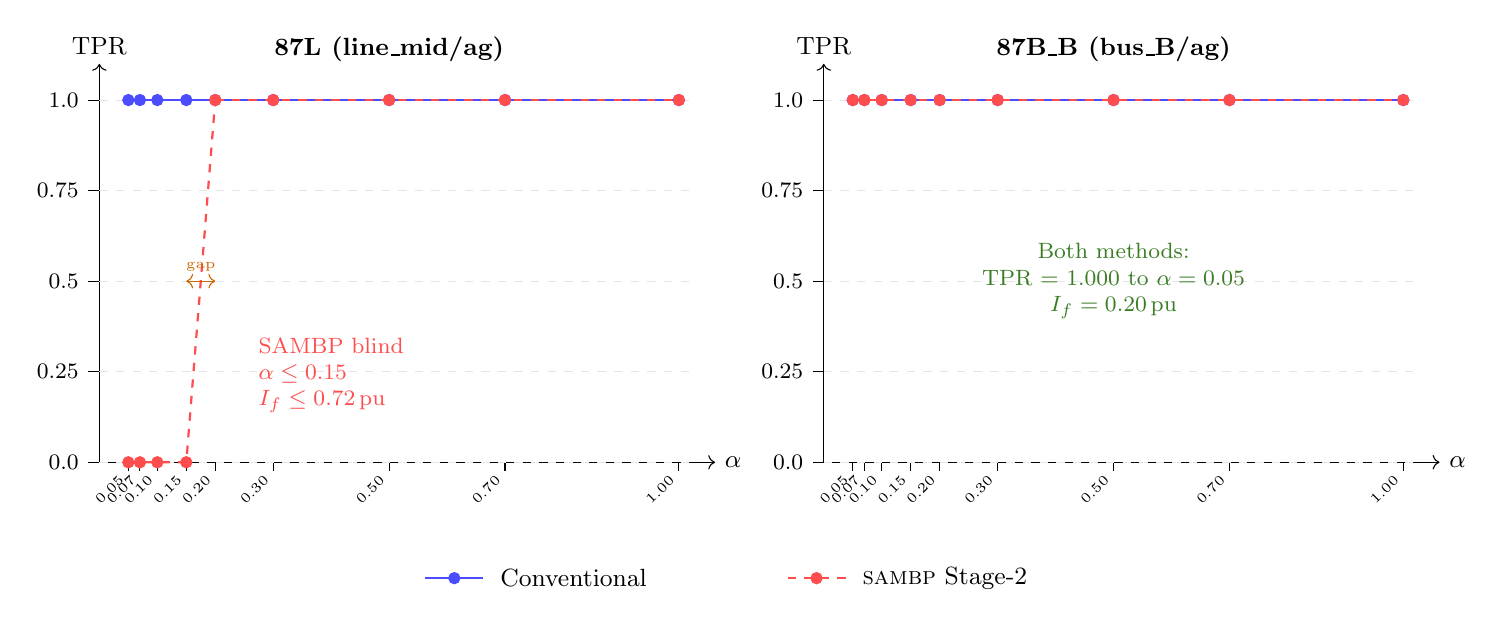
\begin{tikzpicture}[scale=0.92]

% Shared axis setup
% X axis: I_f scaled [pu] from 0 to 10, log-ish but linear for clarity
% Use linear x mapped from alpha × I_f_nom

%-------------------------------------------------------------------
% Left plot: 87L ag (line_mid/ag — I_f_nom=4.8 pu)
%   alpha:  1.00  0.70  0.50  0.30  0.20  0.15  0.10  0.07  0.05
%   I_f:    4.8   3.36  2.40  1.44  0.96  0.72  0.48  0.336 0.24
%   conv:   1     1     1     1     1     1     1     1     1
%   sambp:  1     1     1     1     1     0     0     0     0
%
% Normalised X: I_f / I_f_nom, so X ∈ [0.05, 1] → map to 0..8 cm

\begin{scope}[xshift=0cm]

% Axes
\draw[->] (0,0)--(8.5,0) node[right,font=\small]{$\alpha$};
\draw[->] (0,0)--(0,5.5) node[above,font=\small]{TPR};

% X ticks (alpha values)
\foreach \a/\lbl in {8.0/1.00, 5.6/0.70, 4.0/0.50, 2.4/0.30, 1.6/0.20, 1.2/0.15, 0.8/0.10, 0.56/0.07, 0.4/0.05}{
    \draw (\a,0)--(\a,-0.12) node[below,font=\tiny,rotate=45,anchor=east]{\lbl};
}
% Y ticks
\foreach \y/\v in {0/0.0,1.25/0.25,2.5/0.5,3.75/0.75,5.0/1.0}{
    \draw (0,\y)--(-0.15,\y) node[left,font=\footnotesize]{\v};
    \draw[gray!20,dashed](0,\y)--(8.2,\y);
}

% Conv line (always 1.000)
\draw[blue!70,thick]
  (0.4,5.0)--(0.56,5.0)--(0.8,5.0)--(1.2,5.0)--(1.6,5.0)
  --(2.4,5.0)--(4.0,5.0)--(5.6,5.0)--(8.0,5.0);
\foreach \x in {0.4,0.56,0.8,1.2,1.6,2.4,4.0,5.6,8.0}{
    \filldraw[blue!70] (\x,5.0) circle(2.2pt);}

% SAMBP line (drops to 0 at alpha<=0.15)
%  alpha: 1.00→5.0, 0.70→5.0, 0.50→5.0, 0.30→5.0, 0.20→5.0, 0.15→0.0, ...
\draw[red!70,thick,dashed]
  (1.6,5.0)--(2.4,5.0)--(4.0,5.0)--(5.6,5.0)--(8.0,5.0);
\draw[red!70,thick,dashed]
  (0.4,0.0)--(0.56,0.0)--(0.8,0.0)--(1.2,0.0)--(1.6,5.0);
\foreach \x/\y in {8.0/5.0,5.6/5.0,4.0/5.0,2.4/5.0,1.6/5.0,1.2/0.0,0.8/0.0,0.56/0.0,0.4/0.0}{
    \filldraw[red!70] (\x,\y) circle(2.2pt);}

% Threshold arrow
\draw[<->,orange!80!black,thin] (1.2,2.5)--(1.6,2.5)
  node[midway,above,font=\tiny]{gap};

% Label
\node[font=\small\bfseries] at (4.0,5.7) {87L (line\_mid/ag)};
\node[font=\footnotesize,align=left,text=red!70] at (3.2,1.2)
  {SAMBP blind\\$\alpha \leq 0.15$\\$I_f \leq 0.72$\,pu};

\end{scope}

%-------------------------------------------------------------------
% Right plot: 87B ag (bus_B/ag — I_f_nom=4.0 pu)
%   alpha:   1.00  0.70  0.50  0.30  0.20  0.15  0.10  0.07  0.05
%   I_f:     4.0   2.8   2.0   1.2   0.8   0.6   0.4   0.28  0.20
%   conv:    1     1     1     1     1     1     1     1     1
%   sambp:   1     1     1     1     1     1     1     1     1

\begin{scope}[xshift=10cm]

\draw[->] (0,0)--(8.5,0) node[right,font=\small]{$\alpha$};
\draw[->] (0,0)--(0,5.5) node[above,font=\small]{TPR};

\foreach \a/\lbl in {8.0/1.00,5.6/0.70,4.0/0.50,2.4/0.30,1.6/0.20,1.2/0.15,0.8/0.10,0.56/0.07,0.4/0.05}{
    \draw (\a,0)--(\a,-0.12) node[below,font=\tiny,rotate=45,anchor=east]{\lbl};
}
\foreach \y/\v in {0/0.0,1.25/0.25,2.5/0.5,3.75/0.75,5.0/1.0}{
    \draw (0,\y)--(-0.15,\y) node[left,font=\footnotesize]{\v};
    \draw[gray!20,dashed](0,\y)--(8.2,\y);
}

% Both lines at 1.000 always
\draw[blue!70,thick]
  (0.4,5.0)--(0.56,5.0)--(0.8,5.0)--(1.2,5.0)--(1.6,5.0)
  --(2.4,5.0)--(4.0,5.0)--(5.6,5.0)--(8.0,5.0);
\foreach \x in {0.4,0.56,0.8,1.2,1.6,2.4,4.0,5.6,8.0}{
    \filldraw[blue!70] (\x,5.0) circle(2.2pt);}

\draw[red!70,thick,dashed]
  (0.4,5.0)--(0.56,5.0)--(0.8,5.0)--(1.2,5.0)--(1.6,5.0)
  --(2.4,5.0)--(4.0,5.0)--(5.6,5.0)--(8.0,5.0);
\foreach \x in {0.4,0.56,0.8,1.2,1.6,2.4,4.0,5.6,8.0}{
    \filldraw[red!70] (\x,5.0) circle(2.2pt);}

\node[font=\small\bfseries] at (4.0,5.7) {87B\_B (bus\_B/ag)};
\node[font=\footnotesize,align=center,text=OliveGreen] at (4.0,2.5)
  {Both methods:\\TPR = 1.000 to $\alpha = 0.05$\\$I_f = 0.20$\,pu};

\end{scope}

% Shared legend
\draw[blue!70,thick] (4.5,-1.6)--(5.3,-1.6);
\filldraw[blue!70] (4.9,-1.6) circle(2.2pt);
\node[right,font=\small] at (5.4,-1.6) {Conventional};
\draw[red!70,thick,dashed] (9.5,-1.6)--(10.3,-1.6);
\filldraw[red!70] (9.9,-1.6) circle(2.2pt);
\node[right,font=\small] at (10.4,-1.6) {\textsc{sambp} Stage-2};

\end{tikzpicture}

  \caption{TPR vs.\ fault current scale factor $\alpha$.
    \emph{Left}: 87L line differential — \SAMBP{} Stage-2 loses
    detection at $\alpha \leq 0.15$ while the conventional relay
    detects to $\alpha = 0.05$.
    \emph{Right}: 87B bus differential — both methods achieve
    TPR = 1.000 at all tested levels.}
  \label{fig:margins}
\end{figure}

\subsection{Over-Current Relay (OC)}

The OC relay detection boundary is analytically determined by the pickup
threshold $I_{\rm OC,pickup} = 1.5$~pu (set in TR-05) and the fault
current RMS.

\begin{table}[ht]
\centering
\caption{OC relay detection results at bus\_C\_load.
  The OC relay is identical in conventional and \SAMBP{} paths
  (Stage-2 gate not applied to OC).}
\label{tab:oc}
\begin{tabular}{cccc}
\toprule
$\alpha$ & $I_f$ [pu] & $I_{\rm rms}$ [pu] & Trip \\
\midrule
1.00 & 4.348 & 3.074 & Yes \\
0.70 & 3.043 & 2.152 & Yes \\
0.50 & 2.174 & 1.537 & Yes \\
0.30 & 1.304 & 0.922 & \textcolor{warnred}{No (< 1.5)} \\
\bottomrule
\end{tabular}
\end{table}

For the single-phase-to-ground fault (bus\_C\_load/ag), $I_f^{\rm nom}
= 2.609$~pu peak, so $I_{\rm rms}^{\rm nom} \approx 1.845$~pu.  At
$\alpha = 0.70$, $I_{\rm rms} \approx 1.29$~pu $< 1.5$~pu, which
explains the abrupt TPR~=~0 at $\alpha \leq 0.70$ seen in the study.

% ================================================================
\section{Analysis: Why Does 87L Lose Sensitivity Earlier?}
% ================================================================

\subsection{Signal-to-Noise Ratio at the LM Estimator}

The 87L LM estimator receives the differential current
$i_{\rm diff}(t) = i_{\rm near}(t) + i_{\rm far}(t)$ (sum of terminal
currents).  For an internal fault of amplitude $\alpha \cdot I_f^{\rm nom}$,
the fundamental component of $i_{\rm diff}$ is approximately
$\alpha \cdot I_f^{\rm nom}$ pu.

The estimator's residual noise floor is set by:
\begin{itemize}[noitemsep]
  \item Numerical discretisation of the forward model
  \item Charging current from the distributed line capacitance
    (not modelled in the simple line zone model)
  \item DC transient mismatch between the two terminals
\end{itemize}

As $\alpha$ decreases, the signal-to-noise ratio decreases and the LM
estimator converges to solutions with $\fint < 0.60$, triggering the
Stage-2 veto.

\subsection{Comparison with 87B Robustness}

The 87B zone is more robust at low current levels because:
\begin{enumerate}[noitemsep]
  \item Bus differential current is a direct algebraic sum of feeder
    currents — no distributed capacitance or travelling-wave effects.
  \item The bus zone model has no through-current restraint in the
    low-impedance bus topology, so $\Iop \approx I_{\rm diff,fund}$
    directly.
  \item The forward model fits the bus waveform more accurately at
    small amplitudes, keeping $\kappan$ low and $\fint$ close to 1.
\end{enumerate}

\subsection{Implications for HIF Protection Practice}

The 87L detection margin of $\approx 0.72$~pu for phase-to-ground
faults imposes a practical constraint: for a system with rated current
$I_n$ and nominal three-phase fault current $I_f^{\rm 3ph}$, the
minimum detectable fault resistance is approximately:
\begin{equation}
  R_{\rm fault,max}^{\SAMBP} \approx
    \frac{V_{\rm phase}}{0.72 \cdot I_f^{\rm nom}}
    - Z_{\rm line} - Z_{\rm source}
  \label{eq:Rmax}
\end{equation}

For the test network: $I_f^{\rm nom} = 4.8$~pu (ag), $\alpha_{\rm min} =
0.15$, so the minimum detected fault current is $0.15 \times 4.8 =
0.72$~pu.  At a lower fault resistance the conventional relay also fails
to detect (since $I_f$ is then $< \Iopmin$), so the Stage-2 sensitivity
loss only represents a practical degradation in the range $0.20 \leq
I_f \leq 0.72$~pu.

% ================================================================
\section{Detection Margin Summary}
% ================================================================

\begin{table}[ht]
\centering
\caption{HIF detection margin summary across all zones.
  $I_{50}$ = fault current at which TPR first drops below 0.50.
  $I_{\min}^{\rm conv}$ = minimum detected by conventional relay.
  All values in pu of rated current.}
\label{tab:summary}
\begin{tabular}{llcccc}
\toprule
Zone & Scenario &
  $I_f^{\rm nom}$ & $I_{50}^{\rm conv}$ & $I_{50}^{\SAMBP}$ &
  Sensitivity penalty \\
\midrule
87B\_A & bus\_A/3ph & 10.000 & $< 0.50$ & $< 0.50$ & None \\
87B\_A & bus\_A/ag  & 6.000  & $< 0.30$ & $< 0.30$ & None \\
87L   & line\_mid/3ph & 8.000  & $< 0.40$ & 0.56     & $\approx 0.56$~pu \\
87L   & line\_mid/ag  & 4.800  & $< 0.24$ & 0.72     & $\approx 0.72$~pu \\
87B\_B & bus\_B/3ph & 6.667  & $< 0.33$ & $< 0.33$ & None \\
87B\_B & bus\_B/ag  & 4.000  & $< 0.20$ & $< 0.20$ & None \\
87T   & trans\_hv/3ph & 6.667  & $< 0.33$ & $< 0.33$ & None \\
87T   & trans\_hv/ag  & 4.000  & $< 0.20$ & $< 0.20$ & None \\
OC    & bus\_C\_ld/3ph & 4.348 & 1.304    & 1.304    & None (gate inactive) \\
OC    & bus\_C\_ld/ag  & 2.609 & 1.826    & 1.826    & None (gate inactive) \\
\bottomrule
\end{tabular}
\end{table}

% ================================================================
\section{Discussion}
% ================================================================

\subsection{The Selectivity--Sensitivity Trade-Off}

The HIF study quantifies the fundamental trade-off that the Stage-2
gate imposes on the 87L zone.  The gate was designed to reject spurious
trips from through-fault CT saturation and parametric waveform
variation — which it does effectively (FPR~=~0.000 in TR-08 through
TR-10).  The cost is a higher effective detection threshold for
genuine low-current faults.

The trade-off is asymmetric across zones:
\begin{itemize}[noitemsep]
  \item \textbf{87B zones}: no sensitivity penalty because the bus
    differential model fits the waveform accurately at all current levels.
  \item \textbf{87T zone}: same — no penalty.
  \item \textbf{87L zone}: penalty of 0.56--0.72~pu effective threshold
    vs.\ $< 0.24$~pu for the conventional relay.
\end{itemize}

The asymmetry arises because the line zone model has distributed-parameter
effects (line capacitance, travelling wave) that are absent in the lumped
bus and transformer models.  At low current levels the modelling
approximation degrades, reducing $\fint$.

\subsection{Remediation Options}

Three options exist to recover 87L HIF sensitivity:

\begin{enumerate}
  \item \textbf{Magnitude-override extension to 87L.}  Apply the same
    override rule used for 87B (TR-10): if $\hat{I}_{\rm diff,fund} \geq
    I_{\rm ovr}$, bypass the veto.  However, the appropriate $I_{\rm ovr}$
    for 87L must be below the fault current at $\alpha = 0.15$ (0.72~pu),
    suggesting $I_{\rm ovr} \approx 0.30$~pu.  This risks reduced
    selectivity against real CT saturation on through-faults.

  \item \textbf{Improved 87L forward model.}  Replace the lumped-parameter
    line model with a $\Pi$-section equivalent that includes line
    capacitance.  This would improve model accuracy at low current levels
    and increase $\fint$ for genuine internal faults.

  \item \textbf{Dual-threshold gate.}  Use a lower $\fint$ threshold
    ($f_{\rm int,thresh} = 0.40$ instead of 0.60) for the 87L zone,
    reducing the sensitivity penalty while accepting marginally reduced
    selectivity against mild CT saturation.
\end{enumerate}

Option~(2) is preferred as it addresses the root cause (model
approximation quality) rather than the symptom (gate conservatism).
It is recommended as the primary development item following this study.

\subsection{Practical Significance}

In a real power network, high-impedance faults with $I_f < 0.72$~pu
are also below the practical detection limit of conventional OC
protection (typically $\Iopmin \approx 0.20$~pu differential,
$I_{\rm OC,pickup} \approx 0.5$--$1.0$~pu time-overcurrent).  The
HIF range where \SAMBP{} has a sensitivity disadvantage relative to
the conventional \emph{differential} relay is $I_f \in [0.20, 0.72]$~pu
(3.6--36\% of nominal for line\_mid/ag).  Within this range, special
HIF detection algorithms (spectral analysis, pattern recognition) would
be required regardless of the protection scheme.

% ================================================================
\section{Conclusion}
% ================================================================

The HIF sensitivity margin study establishes quantitative lower
bounds for \SAMBP{} detection capability across all four protected zones:

\begin{itemize}
  \item \textbf{87B, 87T}: TPR~=~1.000 maintained to $\alpha = 0.05$
    ($I_f \geq 0.20$~pu).  No sensitivity penalty vs.\ conventional relay.

  \item \textbf{87L}: Stage-2 gate raises effective detection threshold
    from $< 0.24$~pu (conventional) to $0.56$~pu (3ph) / $0.72$~pu (ag).
    Root cause: low-SNR differential at reduced fault levels produces
    ambiguous LM solutions with $\fint < 0.60$.

  \item \textbf{OC}: Detection threshold determined analytically by the
    pickup threshold (1.5~pu RMS) and nominal fault current.
\end{itemize}

The 87L sensitivity penalty represents a quantified selectivity--sensitivity
trade-off.  Remediation via an improved distributed-parameter 87L forward
model is recommended.

\bigskip\noindent\textbf{Availability.}
Script: \texttt{sambp/sambp\_system/run\_hif\_study.py} (seed~2026).

\newpage
\bibliographystyle{plainnat}
\bibliography{references11}

\end{document}
